\pagebreak
\chapter{Classification Results \& Discussion}
\label{sec:results}

%\section{Data Analysis - Results}

\section{Category-Secific Baseline Brain Activation \textit{(UPA)} - Results}

The average signal for faces in the \gls{FFA} is unexpectedly low (see \autoref{fig:upa_ffa}). However, this does not compromise the efficacy of \gls{MVPA}, as successful classification of category-specific signals relies on their patterns' distinctiveness from other signals, regardless of whether this distinction is due to signal strength or relative weakness. Nevertheless, this finding warrants further investigation.

\vspace{2pt}

\begin{figure}[htbp]
 	\centering
	\begin{subfigure}{0.49\textwidth}
		\centering
		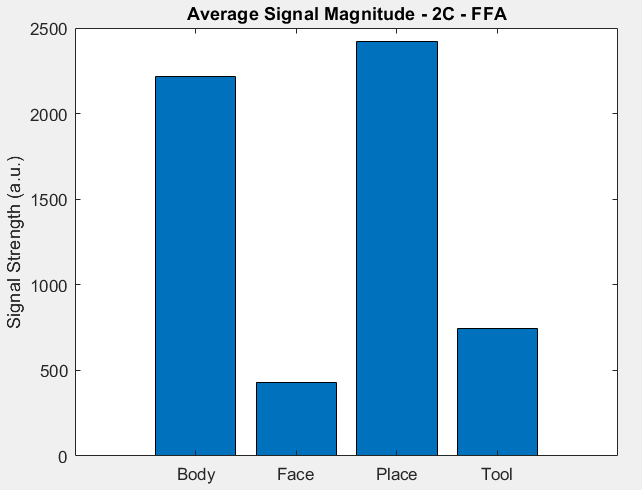
\includegraphics[width = 0.8\textwidth, height = 5cm]{assets/images/upa_2C_ffa.png}
		\caption{Average Magnitude of Brain Activation in the \gls{FFA} Across Different Stimulus Categories in the \gls{2C} Analysis.}
		\label{fig:upa_ffa_2C}
	\end{subfigure}
	\hfill
	\begin{subfigure}{0.49\textwidth}
		\centering
	 	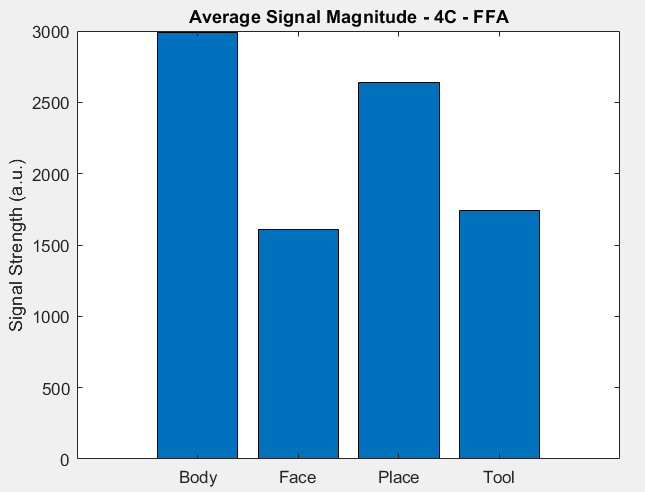
\includegraphics[width = 0.8\textwidth, height = 5cm]{assets/images/upa_4C_ffa.png}
		\caption{Average Magnitude of Brain Activation in the \gls{FFA} Across Different Stimulus Categories in the \gls{4C} Analysis.}
		\label{fig:upa_ffa_4C}
	\end{subfigure}
	\caption[Activation Magnitude Per Stimulus Category \textit{(UPA)} Bar Plots for the FFA]{Bar Plots Showing the Mean Activation for Each Stimulus Category Across the \gls{FFA}.}
 	\label{fig:upa_ffa}
\end{figure}

\vspace{2pt}

\begin{wrapfigure}{r}{0.4\textwidth}
    \centering
    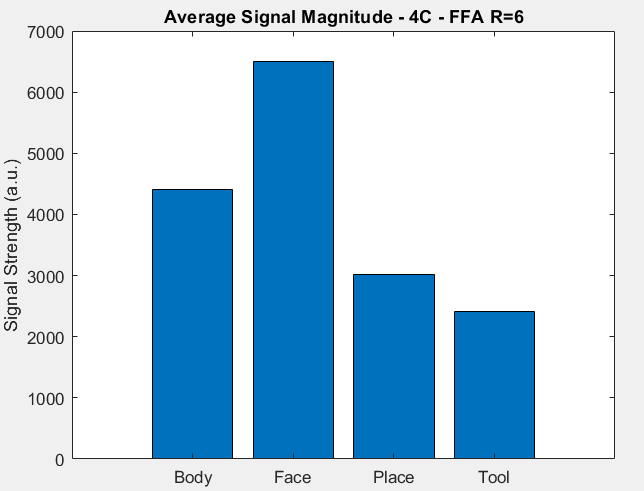
\includegraphics[width = 0.4\textwidth, height = 4.7cm]{assets/images/upa_4C_ffa_6.png}
    \caption[Activation Magnitude Per Stimulus Category \textit{(UPA)} Bar Plots for the FFA Centrally]{Bar Plots Showing the Mean Activation for Each Stimulus Category Across the \gls{FFA} When Mask Radius is 6.}
    \label{fig:upa_ffa_6}
\end{wrapfigure}

Examining the \gls{WM} task battery from which the data was derived, we observe that Faces were presented immediately after Bodies in the first instance and after Places in the second, never directly following a fixation phase. This sequence likely resulted in residual signals from the preceding stimulus categories, which could explain the magnitude observed for Bodies and Places. However, this does not account for the higher magnitude of Tools, which, theoretically, should not surpass that of Faces. A closer examination of the more central portion of the \gls{FFA} (see \autoref{fig:upa_ffa_6}), where residual overlap from other sources is minimized, reveals the expected signal profile: Faces show the highest activation magnitude, with Tools displaying roughly the same relative amplitude. This observation supports the earlier hypothesis and confirms that \gls{MVPA} can proceed using the initial, full \gls{FFA} mask.

In contrast, the signal in the \gls{PPA} is significantly higher for places than other stimuli (see \autoref{fig:upa_ppa}) throughout the whole region. The category-specific signals also tend to be ranked according to the proximity of their corresponding areas to the \gls{PPA}, suggesting that the differences in baseline signal may be due to overlap from place stimuli.

\begin{figure}[htbp]
 	\centering
	\begin{subfigure}{0.49\textwidth}
		\centering
		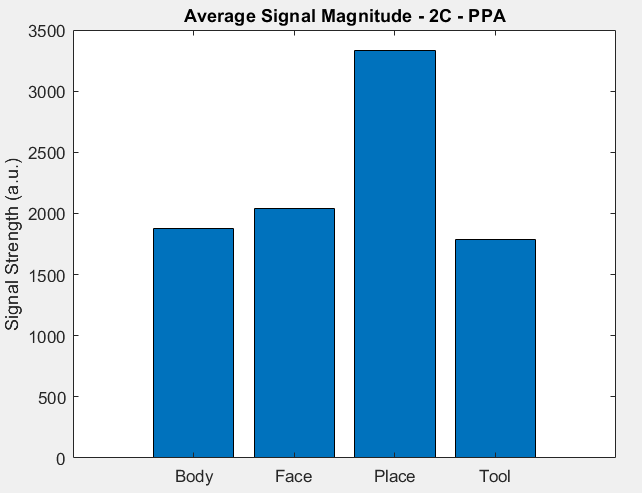
\includegraphics[width = 0.8\textwidth, height = 5cm]{assets/images/upa_2C_ppa.png}
		\caption{Average Magnitude of Brain Activation in the \gls{PPA} Across Different Stimulus Categories in the \gls{2C} Analysis..}
		\label{fig:upa_ppa_2C}
	\end{subfigure}
	\hfill
	\begin{subfigure}{0.49\textwidth}
		\centering
	 	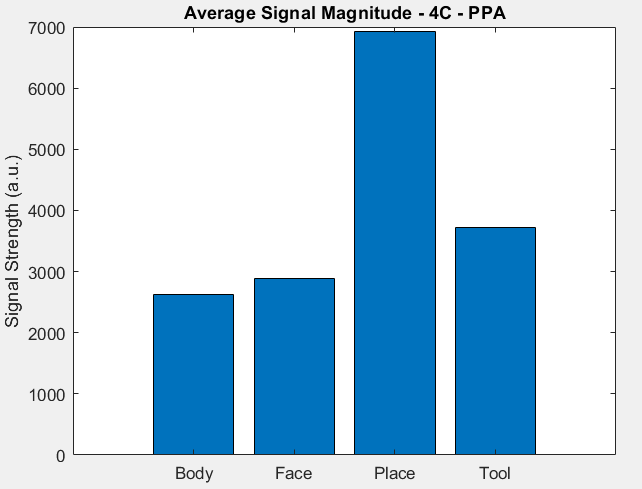
\includegraphics[width = 0.8\textwidth, height = 5cm]{assets/images/upa_4C_ppa.png}
		\caption{Average Magnitude of Brain Activation in the \gls{PPA} Across Different Stimulus Categories in the \gls{4C} Analysis..}
		\label{fig:upa_ppa_4C}
	\end{subfigure}
	\caption[Activation Magnitude Per Stimulus Category \textit{(UPA)} Bar Plots for the PPA]{Bar Plots Showing the Mean Activation for Each Stimulus Category Across the \gls{PPA}.}
 	\label{fig:upa_ppa}
\end{figure}

Notably, Places were presented once after a fixation phase and once after Tools, ensuring that the resulting signal is more canonical. As a result, the classifier is likely to perform better for place stimuli, although this will ultimately be confirmed or disproven by \gls{MVPA}.




%%% Start of FFA %%%




\section{Fusiform Face Area MVPA - Results}

\glsreset{FFA}
These are the classifier's performance results for the \gls{FFA}, analyzed across different variables.

\subsection{Chunks Per Subject \textit{(FFA)} - Results}

Using \gls{2C} data, the classifier achieved an optimal mean accuracy of 70\% across 3000 folds in the \gls{FFA}, while performance with \gls{4C} data capped at 61.9\%. The distributions of accuracies across folds were tested for normality, and a Lilliefors test confirmed that the data did not follow a normal distribution, with p-values of $1^{-3}$ for both datasets. Given that the two distributions also differed in variances, as shown by a two-sample F-test with a p-value of $<10^{-16}$, a Wilcoxon Rank-Sum test was conducted. The discrepancy between means was found to be statistically significant, with a p-value of $<10^{-16}$, undoubtedly confirming that the different approaches yielded distinct results and that the two analyses should be examined separately.

\subsection{Outlier Subjects \textit{(FFA)} - Results}
\label{subs:res_outliers_ffa}

After the classifier ran on each subject's data separately, using the maximum number of folds (4), the mean accuracies for each subject were calculated. As expected, these accuracies were generally lower than those obtained when the classifier was fed larger datasets. When all 20 subjects were included individually, the mean accuracy was 50\%, with a median value of 56.3\% (see \autoref{fig:per_subj_all_ffa}). However, two cases stood out immediately: Subject 100408 had a surprising accuracy of 0\%, and Subject 116524 showed an accuracy of 6.25\%. Given that the classifier completely failed to identify category-specific neural patterns in the first subject's data, it was assumed that the data was faulty for this analysis, and this subject was excluded from further steps. However, no robust reasoning was found to classify the second subject as an outlier, so they were included in the analysis.

\begin{figure}[htbp]
 	\centering
	\begin{subfigure}{0.49\textwidth}
		\centering
		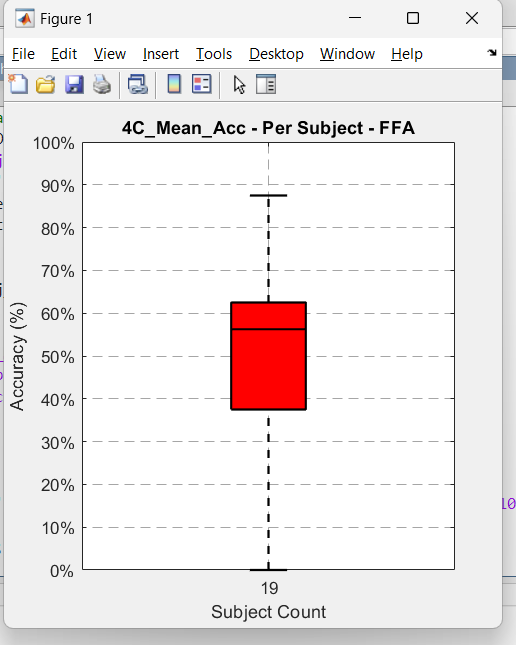
\includegraphics[width = 0.9\textwidth, height = 5cm]{assets/images/per_subj_4C_20_ffa.png}
		\caption{Boxplot Illustrating the Distribution of Initial Accuracy Across Individual Subjects.}
		\label{fig:per_subj_all_ffa}
	\end{subfigure}
	\hfill
	\begin{subfigure}{0.49\textwidth}
		\centering
	 	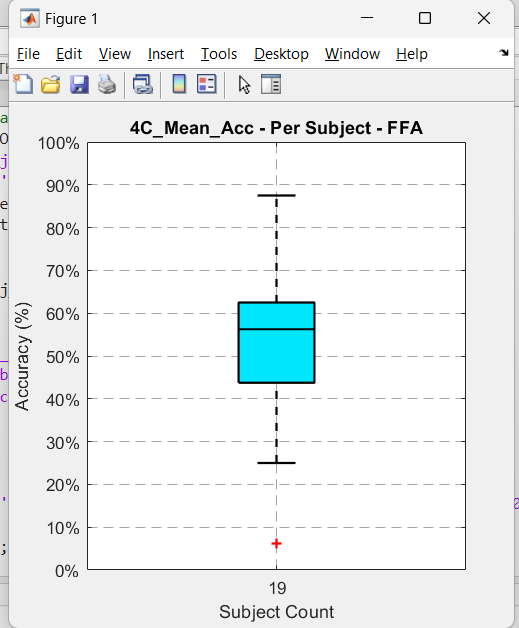
\includegraphics[width = 0.9\textwidth, height = 5cm]{assets/images/per_subj_4C_19_ffa.png}
		\caption{Boxplot Illustrating Accuracy Variance Across Individual Subjects After Excluding Outliers.}
		\label{fig:per_subj_19_ffa}
	\end{subfigure}
	\caption[Individual Subjects' Accuracies Boxplots for the FFA]{Boxplots Generated from the 'Per Subject' Analysis in the \gls{FFA}.}
 	\label{fig:per_subj_ffa}
\end{figure}

Once the outlier was removed, the mean accuracy for analyses involving one subject at a time increased to 52.6\%, with the median remaining constant (see \autoref{fig:per_subj_19_ffa}). Normally, this was still lower than the classifier's maximum potential accuracy of 61.9\%, which can be attributed to the low fold count used in these analyses. These results clearly indicate that screening for outlier subjects is crucial, as their inclusion can significantly impact the classifier's performance, particularly when working with smaller subject pools.

\subsection{Fold Count \textit{(FFA)} - Results}

The initial analysis, which focused on high fold counts, showed that accuracy stabilized to the second decimal point by 250 folds for both \gls{4C} and \gls{2C} analyses. This stability was reflected in the standard deviations of the distributions, which were 0.15\% for \gls{4C} and 0.17\% for \gls{2C}. In both cases, accuracy was slightly overestimated in the lower fold range of 250–1000, but eventually plateaued over 2500 folds, reaching 61.9\% for \gls{4C} and 70\% for \gls{2C}. These values represent the classifier's true accuracy and serve as the benchmarks to aim for in more practical, lower fold count analyses.

\begin{figure}[htbp]
 	\centering
	\begin{subfigure}{0.49\textwidth}
		\centering
		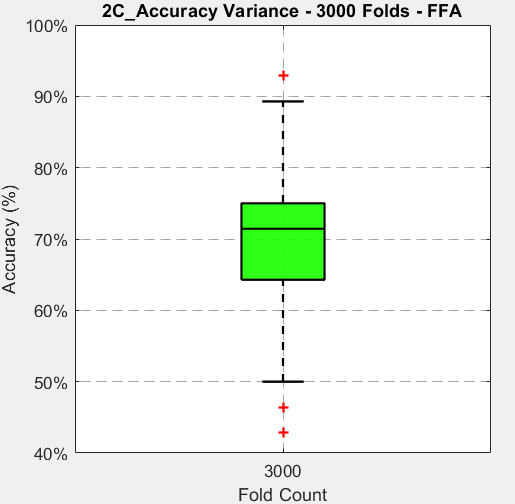
\includegraphics[width = 0.9\textwidth, height = 5cm]{assets/images/box_2C_3000_ffa.png}
		\caption{Accuracy Variance Across 3000 Folds for \gls{2C} Data.}
		\label{fig:2C_3000_ffa}
	\end{subfigure}
	\hfill
	\begin{subfigure}{0.49\textwidth}
		\centering
	 	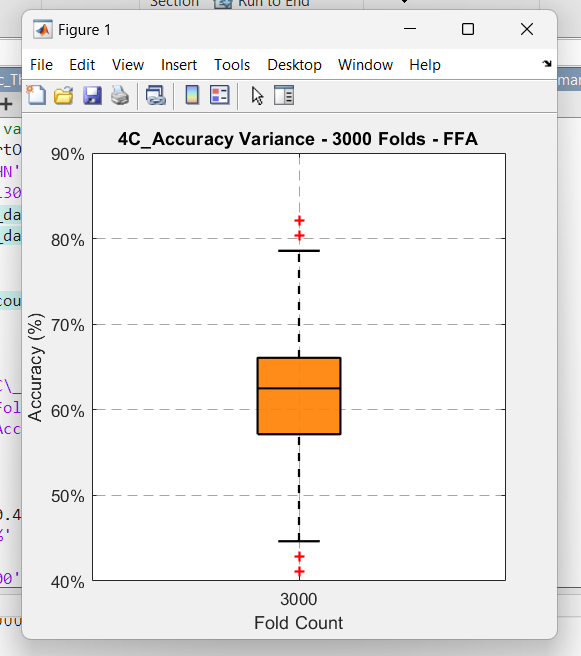
\includegraphics[width = 0.9\textwidth, height = 5cm]{assets/images/box_4C_3000_ffa.png}
		\caption{Accuracy Variance Across 3000 Folds for \gls{4C} Data.}
		\label{fig:4C_3000_ffa}
	\end{subfigure}
	\caption[Accuracies Across 3000 Folds Boxplots For The FFA]{Boxplots Produced During the 'High Number of Folds' Analysis in the \gls{FFA}.}
 	\label{fig:fold_HN_ffa}
\end{figure}

Furthermore, \autoref{fig:fold_HN_ffa} presents a boxplot for both analyses, illustrating the spread of accuracies across all 3000 folds. This distribution of partitions drives the classifier to its benchmark performance. To establish a practical fold count, the partitioning scheme distribution should mimic the one shown in the boxplot. This rationale led to the optimal practical fold count values being set at 69 for \gls{2C} and 68 for \gls{4C}.

\begin{figure}[htbp]
 	\centering
	\begin{subfigure}{0.49\textwidth}
		\centering
		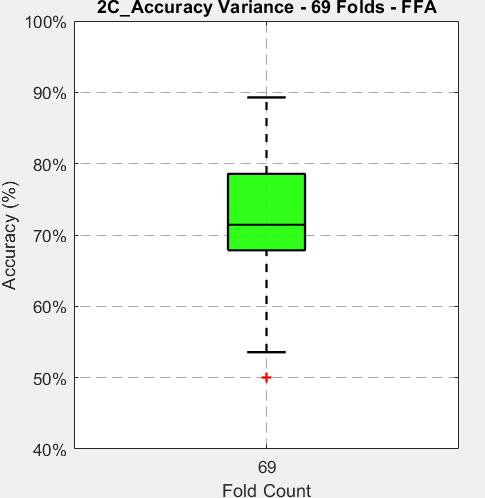
\includegraphics[width = 0.9\textwidth, height = 5cm]{assets/images/box_2C_69_ffa.png}
		\caption{Accuracy Variance Across the Optimal 69 Folds for \gls{2C} Data.}
		\label{fig:2C_69_ffa}
	\end{subfigure}
	\hfill
	\begin{subfigure}{0.49\textwidth}
		\centering
	 	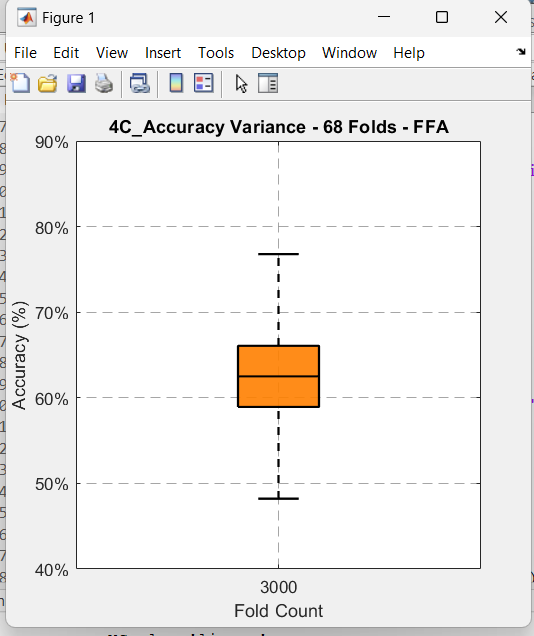
\includegraphics[width = 0.9\textwidth, height = 5cm]{assets/images/box_4C_68_ffa.png}
		\caption{Accuracy Variance Across the Optimal 68 Folds for \gls{4C} Data.}
		\label{fig:4C_68_ffa}
	\end{subfigure}
	\caption[Accuracies At Optimal Fold Count Boxplots For The FFA]{Boxplots Produced During the 'Practical Fold Count' Analysis in the \gls{FFA}.}
 	\label{fig:fold_ffa}
\end{figure}

The boxplots illustrated in \autoref{fig:fold_ffa} demonstrate distributions that closely resemble those obtained from the 3000-fold count analysis. These results indicate that the practical fold count approach provides both high accuracy and efficiency, making it a viable alternative for repeated analyses without compromising on the classifier's performance. The similarity in distributions confirms that reducing the number of folds to a more manageable level does not significantly affect the accuracy of the results.

\subsection{Subject Count \textit{(FFA)} - Results}

In the context of the \gls{2C} analysis, \autoref{fig:count_2C_ffa} shows that with just 2 subjects included, the classifier is already performing at a 50\% success rate. As more subjects are added, accuracy naturally increases, oscillating within the 65-70\% range, and eventually approaches the classifier's true potential accuracy of 70\% with 19 subjects included. The only truly irregular data point occurs at 4 subjects, where the classifier achieves a 78.1\% success rate. This anomaly can be attributed to the low number of data points in the analysis at this stage, combined with the necessarily low fold counts used in low subject counts analyses, and does not reflect a realistic performance for the classifier.

\begin{figure}[htbp]
 	\centering
	\begin{subfigure}{0.49\textwidth}
		\centering
		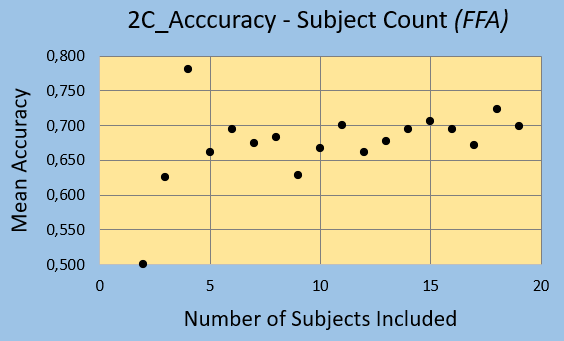
\includegraphics[width = 0.9\textwidth, height = 5cm]{assets/images/subj_count_2C_ffa.png}
		\caption{Accuracy Variance Across Different Subject Counts for \gls{2C} Data.}
		\label{fig:count_2C_ffa}
	\end{subfigure}
	\hfill
	\begin{subfigure}{0.49\textwidth}
		\centering
	 	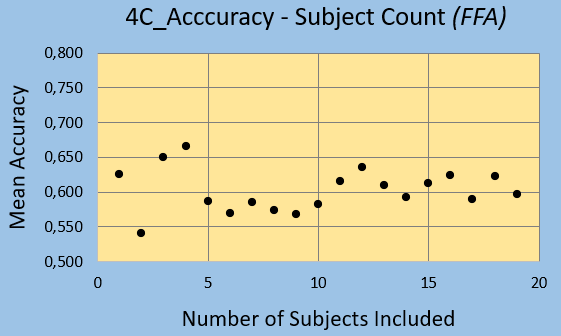
\includegraphics[width = 0.9\textwidth, height = 5cm]{assets/images/subj_count_4C_ffa.png}
		\caption{Accuracy Variance Across Different Subject Counts for \gls{4C} Data.}
		\label{fig:count_4C_ffa}
	\end{subfigure}
	\caption[Accuracies Across Subject Counts For The FFA]{Data Produced During the 'Subject Count' Analysis in the \gls{FFA}.}
 	\label{fig:count_ffa}
\end{figure} 

The same behavior is observed for the \gls{4C} analysis (see \autoref{fig:count_4C_ffa}). The overly high accuracy pattern at 3 and 4 subjects is repeated, further supporting the idea that brain activation patterns and partitioning schemes at this stage are overly favorable for the classifier. Additionally, another irregular point is observed at a subject count of 1, which was not feasible in the previous analysis. In this case, the fold count is only 4, and the potential performance outcomes are too limited to be truly representative. Therefore, interpreting the data at such low subject counts holds little value.

In both cases, accuracy appears to reach realistic values with at least 5 subjects, showing 66.1\% compared to the optimal 69.9\% for the \gls{2C} analysis and 58.7\% compared to the optimal 59.7\% for the \gls{4C} analysis.

The reasons behind this behavior of the classifier can only be speculated, as the baseline signal appears irregular (see \autoref{fig:upa_ffa}). A likely explanation is that the rapid stabilization of the classifier's accuracy is not so much a positive sign, as it indicates not that the classifier achieves high success rates at low subject counts but instead that it fails to increase success rate with additional data points. This could be due to the mixed nature of the baseline signal resulting in the disparity among stimuli categories being potentially, yet unpredictably, extenuated as more subjects are included in the analysis.





%%% Switch from FFA to PPA %%%





\section{Parahippocampal Place Area MVPA - Results}

\glsreset{PPA}
These are the classifier's performance results for the \gls{PPA}, analyzed across different variables.

\subsection{Chunks per Subject \textit{(PPA)} - Results}

In the analysis involving 3000 folds in the \gls{PPA}, the classifier achieved 66.4\% accuracy using \gls{2C} data and 50.6\% with \gls{4C} data, highlighting an even larger gap between the two approaches than in the \gls{FFA}. A Lilliefors test rejected the null hypothesis of normality for both datasets, with p-values of $1^{-3}$. The variance between the two datasets was also significantly different, as confirmed by a two-sample F-test with a p-value of $<10^{-16}$. Finally, the Wilcoxon Rank-Sum test returned a p-value of absolute zero, indicating that it was too low for MATLAB to compute a precise result. This confirms that the two distributions differ significantly and should be investigated separately.

\subsection{Outlier Subjects \textit{(PPA)} - Results}
\label{subs:res_outliers_ppa}

In this case individual accuracy scores were far lower than the classifier's optimal performance, with only three out of twenty cases surpassing it, as indicated by the overall mean accuracy of 32.5\% when all subjects were included with a median of 34.4\% (see \autoref{fig:per_subj_all_ppa}).

\begin{figure}[htbp]
 	\centering
	\begin{subfigure}{0.49\textwidth}
		\centering
		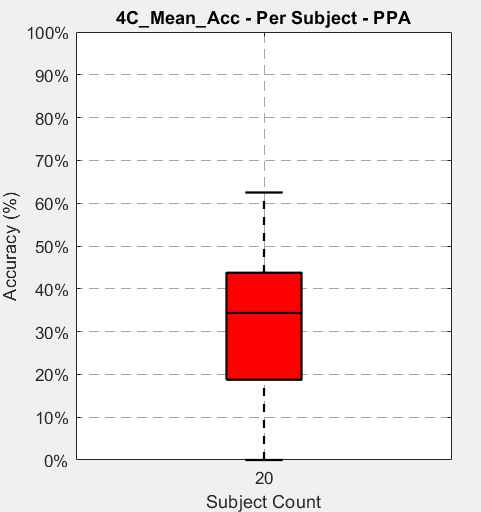
\includegraphics[width = 0.9\textwidth, height = 5cm]{assets/images/per_subj_4C_20_ppa.png}
		\caption{Boxplot Illustrating the Distribution of Initial Accuracy Across Individual Subjects.}
		\label{fig:per_subj_all_ppa}
	\end{subfigure}
	\hfill
	\begin{subfigure}{0.49\textwidth}
		\centering
	 	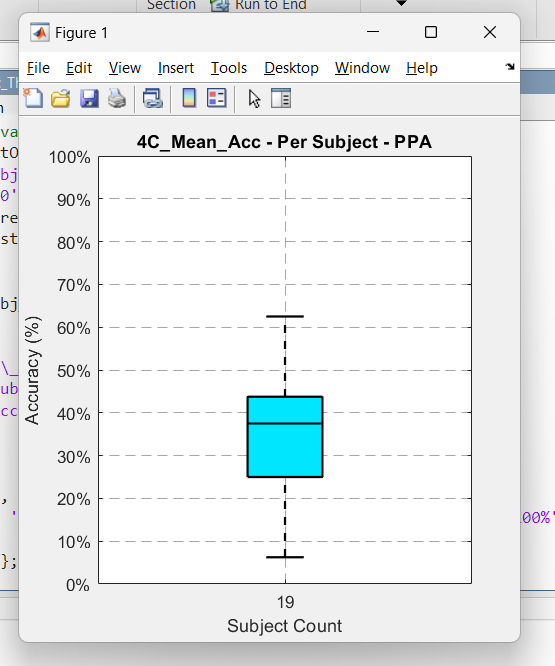
\includegraphics[width = 0.9\textwidth, height = 5cm]{assets/images/per_subj_4C_19_ppa.png}
		\caption{Boxplot Illustrating Accuracy Variance Across Individual Subjects After Excluding Outliers.}
		\label{fig:per_subj_19_ppa}
	\end{subfigure}
	\caption[Individual Subjects' Accuracies Boxplots for the PPA]{Boxplots Generated from the 'Per Subject' Analysis in the \gls{PPA}.}
 	\label{fig:per_subj_ppa}
\end{figure}

The same Subject 100408 produced an accuracy of 0\% again, further enhancing the notion that the specific subject's data potentially includes artifacts or irregularities. Once the outlier subject was excluded, mean accuracy rose to 34.2\% with a median of 37.5\% (see \autoref{fig:per_subj_19_ppa}).

\subsection{Fold Count \textit{(PPA)} - Results}

In both high fold count analyses, accuracy again stabilized to the second decimal point by 250 folds. In the \gls{4C} analysis, there was also stabilization to the third decimal point by 750 folds, with standard deviations of 0.12\% and 0.07\%, for \gls{2C} and \gls{4C} respectively. In the \gls{2C} case, accuracy at low fold counts was slightly lower than the final accuracy ultimately achieved by 2250 folds, which was 66.4\%, while with \gls{4C} data, accuracy remained practically stable throughout, at 50.6\%.

\begin{figure}[htbp]
 	\centering
	\begin{subfigure}{0.49\textwidth}
		\centering
		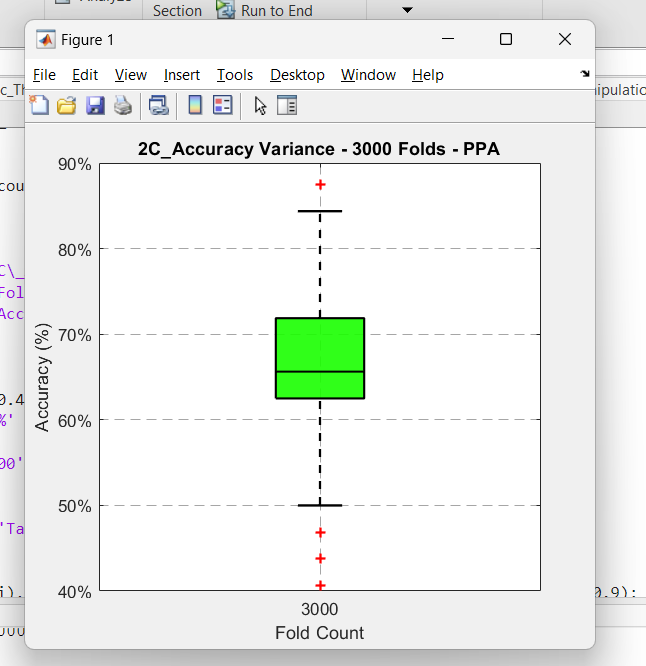
\includegraphics[width = 0.9\textwidth, height = 5cm]{assets/images/box_2C_3000_ppa.png}
		\caption{Accuracy Variance Across 3000 Folds for \gls{2C} Data.}
		\label{fig:2C_3000_ppa}
	\end{subfigure}
	\hfill
	\begin{subfigure}{0.49\textwidth}
		\centering
	 	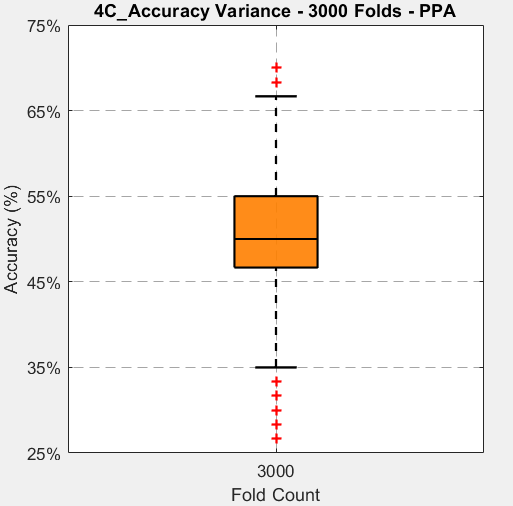
\includegraphics[width = 0.9\textwidth, height = 5cm]{assets/images/box_4C_3000_ppa.png}
		\caption{Accuracy Variance Across 3000 Folds for \gls{4C} Data.}
		\label{fig:4C_3000_ppa}
	\end{subfigure}
	\caption[Accuracies Across 3000 Folds Boxplots For The PPA]{Boxplots Produced During the 'High Number of Folds' Analysis in the \gls{PPA}.}
 	\label{fig:fold_HN_ppa}
\end{figure}

\autoref{fig:fold_HN_ppa} showcases the spread of accuracies across all 3000 folds for both analyses, indicating the distribution that should be sought after at low fold counts as well. With these in mind, the optimal practical fold count for \gls{2C} was set at 49 and for \gls{4C} at 62.

\begin{figure}[htbp]
 	\centering
	\begin{subfigure}{0.49\textwidth}
		\centering
		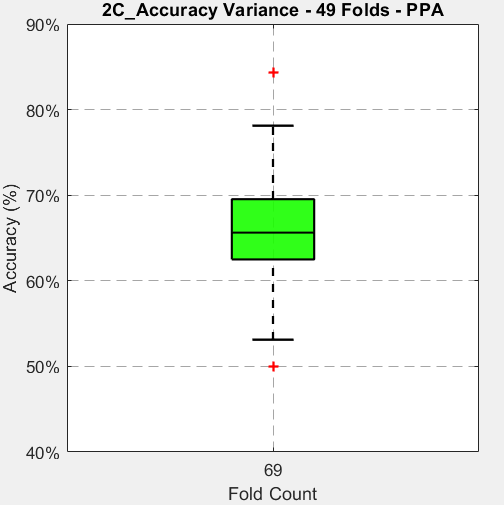
\includegraphics[width = 0.9\textwidth, height = 5cm]{assets/images/box_2C_49_ppa.png}
		\caption{Accuracy Variance Across the Optimal 49 Folds for \gls{2C} Data.}
		\label{fig:2C_49_ppa}
	\end{subfigure}
	\hfill
	\begin{subfigure}{0.49\textwidth}
		\centering
	 	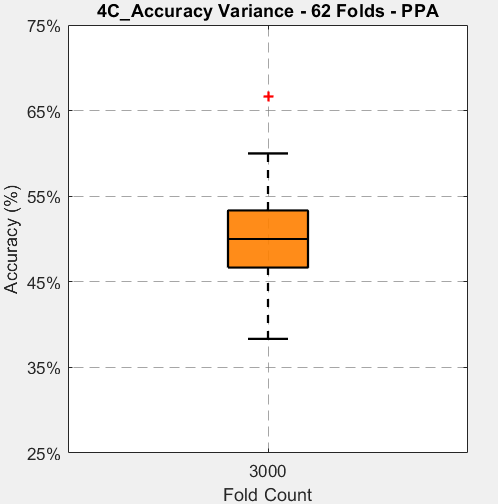
\includegraphics[width = 0.9\textwidth, height = 5cm]{assets/images/box_4C_62_ppa.png}
		\caption{Accuracy Variance Across the Optimal 62 Folds for \gls{4C} Data.}
		\label{fig:4C_62_ppa}
	\end{subfigure}
	\caption[Accuracies At Optimal Fold Count Boxplots For The PPA]{Boxplots Produced During the 'Practical Fold Count' Analysis in the \gls{PPA}.}
 	\label{fig:fold_ppa}
\end{figure}

The accuracy distributions corresponding to the optimal practical fold counts are displayed in \autoref{fig:fold_ppa}. These distributions mirror those obtained from the 3000-fold count analyses, confirming that the classifier's true accuracy can be attained at lower, more  practical fold counts as well.

\subsection{Subject Count \textit{(PPA)} - Results}

In the \gls{2C} analysis (see \autoref{fig:count_2C_ppa}), the classifier begins to perform consistently at around 60\% accuracy once more than 6 subjects are included, gradually increasing to 66.8\% at 15 subjects and then contnueing to oscillate around the final value of 66.4\%. At lower subject counts, performance improves rapidly in a linear fashion as more subjects are added, with the only anomaly occurring at 5 subjects, where a notably precise accuracy of 67.5\% is achieved. This subject count could be leveraged for extremely fast, efficient, and relatively accurate analyses, requiring manipulation of just 20 patterns in total.

\begin{figure}[htbp]
 	\centering
	\begin{subfigure}{0.49\textwidth}
		\centering
		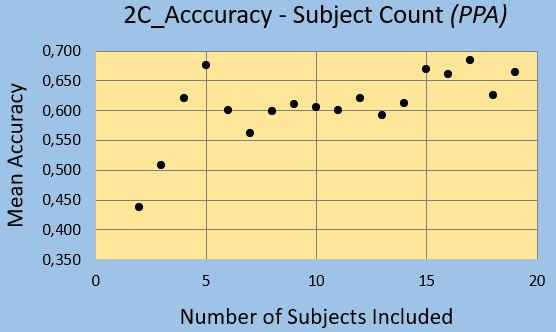
\includegraphics[width = 0.9\textwidth, height = 5cm]{assets/images/subj_count_2C_ppa.png}
		\caption{Accuracy Variance Across Different Subject Counts for \gls{2C} Data.}
		\label{fig:count_2C_ppa}
	\end{subfigure}
	\hfill
	\begin{subfigure}{0.49\textwidth}
		\centering
	 	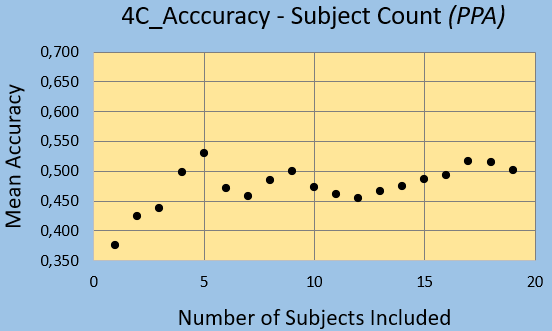
\includegraphics[width = 0.9\textwidth, height = 5cm]{assets/images/subj_count_4C_ppa.png}
		\caption{Accuracy Variance Across Different Subject Counts for \gls{4C} Data.}
		\label{fig:count_4C_ppa}
	\end{subfigure}
	\caption[Accuracies Across Subject Counts For The PPA]{Data Produced During the 'Subject Count' Analysis in the \gls{PPA}.}
 	\label{fig:count_ppa}
\end{figure} 

A similar pattern is observed in \gls{4C} data (see \autoref{fig:count_4C_ppa}), though in an even more stable manner, with smaller deviations from the mean. The same irregularity at 5 subjects is evident, where accuracy peaks at 52.9\%. Stabilization initially occurs around a low point of 47\% until 14 subjects, after which accuracy slightly oscillates around the final accuracy of 50.1\%.

For \gls{MVPA} in the \gls{PPA}, classifier performance follows a more typical pattern, improving as the number of subjects and data points increases. Performance appears to plateau after about 15 subjects, with the potential for even higher accuracy as more data is included. This can be attributed to the consistent magnitude of brain activation in the \gls{PPA} (as shown in \autoref{fig:upa_ppa}), where the signal for places is significantly higher than for other stimuli. This difference becomes more pronounced with the inclusion of additional subjects and data points, enhancing the classifier's ability to distinguish and accurately classify place-related signals. This effect is even more pronounced in the \gls{4C} case, where the disparity between places and other stimuli categories is greater, leading to fewer fluctuations and a more predictable improvement in the classifier's success rate with added data.




%%% End of PPA %%%




\section{Classification Ideal Parameters}

Below is a summary of the variable sets used by the classifier across different functions.

\subsection{Classifier Maximum Accuracy - Results}

The highest classifier performance, 70\%, was achieved in the \gls{2C} analysis for the \gls{FFA}, using 3000 folds and 19 subjects, with a completion time of 114.1\si{second}. Similarly, with the maximum values of 3000 folds and 19 subjects, the \gls{2C} analysis in the \gls{PPA} achieved a 66.4\% success rate in 117.6\si{second}.

Interestingly, the maximum accuracy was not obtained with the largest datasets but rather from the analysis that combined 2-Back and 0-Back signals for each stimulus category.

\subsection{Classifier Maximum Efficiency - Results}

In the \gls{FFA} \gls{2C} analysis with only 4 subjects and the maximum possible 28 folds, the process completes in just 1.2\si{second}, achieving an accuracy of 78.1\%. As for the \gls{PPA}, in the \gls{2C} analysis using 5 subjects and 45 folds, the classifier reaches a success rate of 67.5\% in just 1.4\si{second}.

While these results cannot be broadly generated with larger datasets, they provide valuable insight into the classifier's potential performance when the data is meticulously screened for artifacts and signals from different stimulus categories are distinctly robust.

\subsection{Classifier Maximum Practicality - Results}

In terms of combining efficiency, precision, and reliability, the \gls{2C} analysis with 11 subjects and 69 folds achieves 70\% accuracy in just 2.6\si{second} for the \gls{FFA}. This matches the success rate of the exhaustive 3000-fold analysis but accomplishes it in a fraction of the time, while also being based on a sufficiently large dataset to ensure reproducible results. In the \gls{PPA}, analyzing \gls{2C} data from 15 subjects at 49 folds yields a classifier accuracy of 66.8\% in 2.9\si{second}. The success pattern is similar to that observed for the \gls{FFA}, although in this case, the data reduction compared to the maximum accuracy analysis was less severe.

These settings should form the basis for the bulk of the analyses, as increasing the magnitude of variables would only demand more computational power and time without offering significant additional benefits.